\documentclass[twoside, 12pt]{iiser-thesis}

%%%%%%%%%%%%%%%%%%%
% Packages/Macros %
%%%%%%%%%%%%%%%%%%%
\usepackage{fullpage}
\usepackage{amssymb,latexsym,amsmath}     % Standard packages
\usepackage{graphicx}
\graphicspath{ {./figures/} }
\usepackage{authblk}
\usepackage{dsfont}
\usepackage{amsthm}
\usepackage{color}
\usepackage{float}
\usepackage[breaklinks=true]{hyperref}
\usepackage[style=apa,
			sorting=nyt,
			date=year,
			bibencoding=utf8,
			isbn=false,
			eprint=false,
			dashed=false,
			uniquelist=false,
			maxbibnames=10,
			minbibnames=1,
			maxcitenames=2,
			uniquename=init,
			giveninits=true,
			useprefix=false,
			minsortnames=1,
			maxsortnames=2]{biblatex}
\renewcommand{\cite}{\parencite}
\bibliography{References}
\setlength{\parskip}{1em}
\usepackage{xurl}
\usepackage{longtable}
\usepackage{caption}
\usepackage{subcaption}
%
% please place your own definitions here and don't use \def but
% THEOREM Environments ---------------------------------------------------

\newtheorem{theo}{{\bf{Theorem}}}[section]
\newtheorem{prop}[theo]{{\bf Proposition}}
\newtheorem{lem}[theo]{{\bf Lemma}}
\newtheorem{coro}[theo]{{\bf Corollary}}
\newtheorem{ex}{{\bf Example}}
\newtheorem{exer}{{\bf Exercise}}
\newtheorem{rem}{{\bf Remark}}[section]
\newtheorem{rems}[rem]{{\bf Remarks}}
\newtheorem{remark}[rem]{Remark}
\newtheorem{defi}{{\bf Definition}}[section]
\newtheorem{defn1}[defi]{Definition}
\newtheorem{defs}[defi]{{\bf Definitions}}
\newtheorem{notation}{{\bf Notation}}[section]
%\newtheorem{mypar}{{\bf }}[section]
%\newcommand{\skp}{\vspace{\baselineskip}}
%%\newcommand{\qed}{\hfill\rule{1.6mm}{1.6mm}}
%\renewcommand{\proof}{\noindent{\bf Proof.\ }}
%\newcommand{\no}{\nonumber}
%\newcommand{\noi}{\noindent}
%\newcommand{\txt}{\textrm}
%\newcommand{\pa}{\partial}
%\newcommand{\ds}{\displaystyle}
%\newcommand{\RR}{\mathbb{R}}
%\newcommand{\si}{\sigma}
%\newcommand{\al}{\alpha}
%\newcommand{\la}{\lambda}
%\newcommand{\La}{\Lambda}
%\newcommand{\calF}{\mathcal{F}}
%\newcommand{\eps}{\varepsilon}
%\newcommand{\ph}{\varphi}
%\newcommand{\sig}{\sigma}
%\newcommand{\tab}{\hspace*{0.3in}}
%\newcommand{\Tab}{\hspace*{1.0in}}
%\newcommand{\vf}{\varphi}
%\newcommand{\del}{\frac{\partial}{\partial t}}
%\newcommand{\vp}{\varepsilon}


\catcode`\@=11
\catcode`\@=12


%%%%%%%%%%%%
% Document %
%%%%%%%%%%%%
%\setcounter{chapter}{-1}

\title{Studying effects of competition on adaptive therapy}


\author{Harshavardhan BV }
\coordinator{Coordinator} \supervisor{Prof. Sutirth Dey} \sdesignation{Professor}
\department{Department of Biology} \reader{Dr. M.S. Madhusudhan}
%\reader{Reader 2}
\dedication{This thesis is dedicated to ?}
\graduationyear{2021}
\academicyear{2020-2021}
\graduationmonth{July}
\def \@bd@lot{0}

\thesisabstract{ Write your  abstract here
}
\acknowledgments{Not more than 250 words}

\begin{document}
	\thesisfront

\chapter{Introduction}

\section{What is Cancer?}
Cancer is a collection of diseases that is usually caused by uncontrolled division of cells with the potential to spread to other parts of the body \cite{cancergov}. Cancer could be caused by extrinsic factors like tobacco usage, excess sun exposure or viral infections, as well as intrinsic factors like inflammation \cite{Trichopoulos,Coussens}. The underlying mechanisms of these causes usually involve genetic mutations or epigenetic changes that alter the DNA, which then trigger a cascade of events that eventually leads to uncontrolled growth of cells \cite{Moolgavkar,Gronbaek}.

Cancer is among the highest non-infectious causes of death among human beings. In the year 2021, over 600,000 deaths are expected to be caused by cancer in the US alone \cite{cancer_stats}. Cancer systems have been of research interest for several decades due to the massive impact it has on human lives. Through such research, we have been able to understand the causes and mechanism of how cancer arises, ways of prevention or early detection of cancer \cite{Loeb,Elmore,Goodman}, and develop new therapies and drugs that can target them more effectively and specifically while minimising unwanted collateral side-effects. While the mortality among some types of cancer have been reduced significantly, we have not been as lucky with other types of cancers and the overall mortality still remains unacceptably high.

\section{Conventional therapy against cancer}
The most common strategies to control cancer that form the frontline of current therapy include radiotherapy, immunotherapy, surgery, and chemotherapy \cite{cancer_therapy}. Radiotherapy involves using ionising radiation to kill cancer cells. The high intensity radiation damages the DNA beyond repair, and this causes the cells to stop dividing and die. However, normal cells are also affected by the ionising radiation and the radiation therefore needs to be focussed to reduce collateral damage \cite{Ahmad}. Surgery involves removal of the tumour using highly invasive procedures. The tumour may be removed in its entirety if it is localised but partial removal may still be required to relieve patients of tumour burden when complete removal would be life threatening \cite{Wyld}. Immunotherapy involves activating the immune system of the body to target the cancer cells for killing. While components of the immune system on their own can detect and kill abnormal cells, cancer cells are able to evolve mechanisms to evade such immune suppression and emerging modes of immunotherapy are attempting to supplement the immune system to better target and fight against these cells \cite{Frankel}. Chemotherapy involves administering cytotoxic drugs to kill cancer cells that frequently target all actively dividing cells, leading to the collateral loss of several stem cell populations \cite{DeVita}. Among more specific kinds of chemotherapy, there are different variants including hormone therapy which suppresses hormones required by cancer cells to survive, and targeted therapy which inhibits specific enzymes or antigens produced by cancer cells \cite{Sawyers,Whitmore}. Occasionally, therapeutic methods may also be devised which use multiple such drugs in combination. Depending on the type and stage of cancer, some of these strategies may not be effective.

Among chemotherapy, the standard clinical protocol, or the Standard of Care (SOC), followed for most cancers is to administer cytotoxic drugs at the maximum tolerated dosage (MTD) \cite{Frei}. The aim of this method is to kill the maximum number of tumour cells as quickly or as early as possible. This minimises the tumour burden quickly and should lead to a better standard of living. Historically however, tumour relapse has been a problem as old as chemotherapy itself. From the earliest days of application of cytotoxic drugs to kill cancer cells, any remission achieved in the clinic has been temporary, and while the time taken for the cancer to grow back varies widely across tumour types, relapse occurs as new populations of cancer cells inevitably emerge \cite{Schilder,Baniel}. Even more problematically, these relapsed tumours have often turned out to be resistant to the cytotoxic drug used earlier and the same drug can therefore no longer be used to control the new cancer population. Drug resistance in cancer, as with bacterial infections, is therefore an active area of research interest, with several approaches under development to predict and treat drug resistance emergence \cite{Mokhtari,Gao,Hall}.

Evolutionary reasoning has been applied extensively to explain and understand the emergence of drug resistance in bacterial populations \cite{Davies}. Like a bacterial population, a tumour would consist of cells with considerable heterogeneity in sensitivity to a cytotoxic drug. Under normal conditions, in the absence of therapy, these cells would compete with each other and keep the number of the resistant phenotype cells in check. Administration of this cytotoxic drug, particularly at a high dose with the goal of maximising cell kill would first kill off the most sensitive cells, which leads to a ``competitive release" of the resistant phenotype \cite{Scott}. The resistant phenotype now grows into the space freed by the killing of sensitive cells without inhibition and takes over the entire population local niche. These resistant phenotypes don’t respond to further dose administered and the therapy fails. This is illustrated in \autoref{comperelease}. It is worth noting that competitive release could happen for other methods of therapy as well, if there are resistant phenotypes for that particular therapy method present in the population.

\begin{figure}[h]
  \centering
  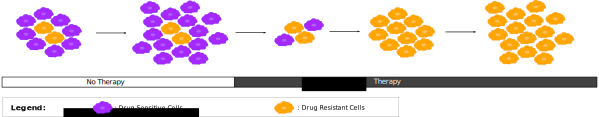
\includegraphics[width=\textwidth]{compe_release}
  \caption{Illustration of competitive release under SOC}
  \label{comperelease}
\end{figure}

\section{Adaptive therapy}
When competitive release happens, one could try to combat the cells with another drug or therapy method. However, these cells could potentially be resistant to the new drug as well and developing new drugs is research intensive. It would therefore be preferable to avoid such competitive release in the first place.

Adaptive therapy (AT) is one such novel approach to therapy under development to avoid competitive release. In AT, the cytotoxic drug is administered at lower and fluctuating doses in which the drug is administered at some lower dose for some duration, which would be followed by a drug holiday \cite{Gatenby}. This doesn’t kill off all the sensitive cells, and allows some fraction of them to remain in the microenvironment to prevent the resistant cells from taking over; this function of the sensitive cell fraction is thought to be due to the pressure of ecological competition they impose on resistant cells by competing with them for space and resources like oxygen. This competitive inhibition of resistant cells by the sensitive ones occurs during the drug holiday, when sensitive cells are not growth-limited by the drug. The tumour burden could then be kept under control as subsequent drug doses counteract the regrowth of sensitive cells during the drug holiday, as illustrated in \autoref{at}. The dosing schedule is therefore a central aspect of AT and must be designed to preserve the competitive inhibition of drug-resistant cells. One of the many regimes envisioned so far in the field uses tumour size as a metric to decide the timing of the dose and when the drug is withdrawn. The challenge with designing AT regimens is to balance the inhibition of resistant phenotype against absolute reduction of the overall tumour size. Adaptive therapy can be influenced by a wide range of factors that affect the dynamics and functioning of the system, and many of these parameters are under active investigation, including but not limited to cell turnover,  phenotypic heterogeneity, spatial constraints and fitness cost for resistance \cite{Strobl,Gallaher,Viossat,Bacevic}.

The promise of tumour control notwithstanding, it is worth noting that AT may not be able to achieve control indefinitely. It only attempts to improve the survival time and/or the time to relapse compared to other regimens and largely ignores the possibility of a cure, sometimes even where the standard of care method might yield better results. The patient has to live with the tumour for the rest of their life and other complications could arise due to this. Models are therefore being developed that could contribute to this decision-making process before therapy. The decision-making model would choose between the aggressive standard-of-care or adaptive therapy to either attempt cure or contain respectively after assessing the probability of cure as well as the risks and complications of maintaining a high tumour burden based on the composition of tumour \cite{Hansen}.

\begin{figure}[h]
  \centering
  \includegraphics[width=\textwidth]{at}
  \caption{Illustration of control under AT}
  \label{at}
\end{figure}

\section{Importance of competition in adaptive therapy}
The only way of controlling the resistant phenotype for a fixed drug under AT is through competition by the sensitive cells. Therefore, the success of AT in containing the tumour depends on the effectiveness of competition between sensitive and resistant cells. It is frequently assumed that resistant cells are required to have an inherent growth disadvantage in the absence of the drug (cost of resistance) for AT to be successful, but it has been shown that the survival time can be prolonged by competition between the cells even without a cost of resistance \cite{Strobl}. Given that competition for resources between cell types can play such a central role in the success of AT regimens, a more detailed examination of how such competitive dynamics could play out would be a valuable addition to the existing literature. More specifically, a description of the competitive interactions between cancer cell types that is framed in terms of explicit resource dynamics along with cell population dynamics is a significant gap worth addressing.

\section{System of Study}
The metastatic castration resistant prostate cancer (mCRPC) was chosen to be the system of study. The mCRPC system already has a history of AT work done on it, although in different contexts \cite{Cunningham,Zhang}.

Prostate cells express androgen receptors (ARs) that require testosterone or its metabolite, 5-dihydrotestosterone to activate. Activated ARs bind to promoters of genes responsible for proliferation \cite{Heinlein}. Without testosterone, proliferation is halted and the cells die of apoptosis. When cancerous cells evolve from prostate cells, the AR mechanism is preserved and the cancer remains testosterone-dependent. However, mutant clones in prostate cancer occur that acquire mutations that allow them to synthesise their own testosterone independent of systemic supply, and these mutant clones are therefore the basis for acquisition of resistance to all forms of castration. Other mutations have also been shown in cancer cells to become entirely testosterone-independent, by acquiring mutations in the AR that make them constitutively active independent of testosterone.

This system is therefore usually modelled as consisting of three different types of cells: $T^+$, $T^p$ and $T^-$. $T^+$ is the baseline population for prostate cancer which requires testosterone for survival and is dependent on systemic supply of the hormone, with no internal sources. The standard therapy for prostate cancer is castration or androgen deprivation therapy (ADT) which blocks external production of testosterone and would kill the $T^+$ cells in a normal castration-sensitive prostate cancer. Castration-resistant prostate cancer cells are modelled as $T^p$ cells that can produce testosterone and sustain the $T^+$ cells. $T^p$ cells are also dependent on testosterone, and they synthesise testosterone from cholesterol through upregulation of the enzyme, CYP17$\alpha$ \cite{Dillard}. Finally, the hormone-independent non-producing fraction of the tumour is modelled as the $T^-$ cells, which do not require testosterone for cell growth. Abiraterone is a drug developed to specifically target castration resistance in prostate cancer that inhibits the CYP17$\alpha$ enzyme and can be effective against both $T^+$ and $T^p$, but would have no effect on $T^-$, as expected based on the functional differences between the three cell types.

\section{Goal of the Project}
This project has the following objectives in the context of adaptive therapy in the castration-resistant prostate cancer system.
\begin{enumerate}
  \item A model must be built of castration-resistant prostate cancer that includes explicit formal descriptions of resource dynamics alongside the dynamics of the three cell types detailed above. The rationale for this is to allow competition in the model to operate through the concentrations of the various resources that constitute the environment. This eliminates the need to estimate values of Lotka-Volterra type competition coefficients that are otherwise difficult to define and interpret based on clinical data.
  \item The model has three cell types which can be studied in stages, starting with two pairs: $T^p-T^-$ and $T^p-T^+$. The third pair, $T^+-T^-$ is a trivial case as $T^+$, with no internal or external sources of testosterone, would go extinct with or without $T^-$. The reason for starting with the pairwise interactions is to come up with a set of simpler observations about how resource concentrations affect competition between two cell types. These simpler observations can then be used to organise and interpret the outcomes of the full three-way competition between $T^p$, $T^+$ and $T^-$. Such a stepwise approach gives us a way to reduce the complexity of a system with three cell types and multiple resources, with each resource produced and consumed differently across the cell types.
  \begin{enumerate}
    \item While the differences of production and consumption of each resource between each cell type is the qualitative basis for interactions between them, these differences do not necessarily constitute competitive strategies, as the status of each cell type with respect to how it interacts with each resource is fixed. For example, if $T^p$ is dependent on testosterone for growth, the magnitude of its sensitivity to a low concentration of testosterone in the environment is the basis of its competitive strategy. While $T^p$ cannot become fully independent of testosterone, the minimum concentration of the hormone required for $T^p$ can be moved around to produce different strengths of competition for the hormone with $T^+$. Strategies of competition are therefore based on the extent to which a given cell type is limited by a resource, given that its mode of dependence is already defined.
    \item Given this definition of competitive strategies, the model can be used to explore competition in two separate contexts, depending on whether all three cell types have the same competitive strategy or each cell type is adopting a strategy unique to that type. Specifically, this is encoded in terms of the level of limitation of a given resource for each cell type. Additionally, both the initial population size and the relative proportion of each cell type in the initial tumour population would have significant effects on the outcomes of competition. Each of these strategies would therefore be studied across a range of population sizes and seeding ratios.
    \item Based on the previous two points, a comprehensive picture of competitive dynamics in the system can be assembled, with an understanding of how this picture is constructed based on the availability and utilisation of various resources.
  \end{enumerate}
  \item The application of therapy affects the ecological balance of this system in very specific ways, and the understanding of competitive interactions in the system based on resource dynamics also allows for outcomes of therapy to be explained in terms of how it affects competition.
  \begin{enumerate}
    \item Standard-of-care (SOC) treatment is the baseline approach against which adaptive therapy (AT) is to be evaluated. SOC involves constant application of the drug at the maximum tolerated dose (MTD). AT design includes at least two parameters-the threshold population sizes at which therapy must be turned on and off, and the gap between these two thresholds. Together, they form the therapy window within which the tumour must be contained. This window can be placed at a large or small population size, and can be wide or narrow. This would form the basis for the standardisation of the AT regimen used for the rest of the model.
    \item Once a standard AT regime is found, it would be applied to the model with all three cell types. As with the study of competition, the standardised AT regimen will be applied to all strategy conditions, across a range of population sizes and seeding densities.
  \end{enumerate}
\end{enumerate}


\chapter{Methods}

\section{System of Equations}
The system of study was modelled using coupled Ordinary Differential Equations (ODEs). The model is based on a logistic framework modified with a dynamic carrying capacity that depends on the environmental conditions. The ``environment" consists of the resources, oxygen and testosterone which have their own equations for production and consumption. We make the simplifying assumption that every other resource required by cells are present in non-limiting concentrations. Additionally, the cell types were assumed to not mutate and hence cannot change their types. No spatial structure is considered and the system is assumed to be well mixed and the resource available in bulk for all the cells.

The ODEs for population size of a cell type is given in \autoref{cell_eq}. The equation is such that the population increases by a maximum growth rate $r_{i,max}$ and reduces by a maximum death rate $\delta_i$. The effective growth rate decreases as the total population approaches a maximum limit while the effective death rate stays the same. This maximum limit for the total population varies between 1 to $K_{i,max}$ and varies depending on the resource availability as a function of the form as given in \autoref{fres_eq} and visualised in \autoref{fig_fres}.\\
For $i \in \{T^+,T^p,T^-\}$
\begin{equation}
  \frac{dy_i}{dt} = r_{i,max}(dtx) y_i (1 - \frac{\sum_j y_j}{1 + K_{i,max} f_i(O_2) f_i(test)} )- \delta_i y_i
  \label{cell_eq}
\end{equation}

The functional dependence on resource $f_i(res) \in [0,1]$. Below the lower limit, $ll_{res,i}$ the function is 0, representative of no growth, and increases linearly above it upto the upper limit, $ul_{res,i}$ and the function saturates to 1, representative of the maximum growth, for any resource levels above that.\\
For $res \in \{O_2,test\}$
\begin{equation}
  f_i(res) = \begin{cases}
  1 &\text{if } ul_{res,i} \leq res \\
  \frac{res-ll_{res,i}}{ul_{res,i}-ll_{res,i}} &\text{if } ll_{res,i} < res < ul_{res,i} \\
  0 &\text{if } res \leq ll_{res,i} \\
  \end{cases}
  \label{fres_eq}
\end{equation}
\begin{figure}[h]
  \centering
  \includegraphics[width=0.5\textwidth]{f_res}
  \caption{$f_i(res)$}
  \label{fig_fres}
\end{figure}

The ODE for oxygen is given in \autoref{o2_eq}. This involves a term for external production that increase oxygen levels constantly at a rate $p_{O_2}$, a term for uptake by all cells where they decrease oxygen levels at a rate $\mu_{O_2,i}$ and a term for decay where oxygen level decreases at a rate $\lambda_{O_2}$.
\begin{equation}
  \frac{dO_2}{dt} = p_{O_2} - \sum_i \mu_{O_2,i} y_i - \lambda_{O_2} O_2
  \label{o2_eq}
\end{equation}

The ODE for testosterone is given in \autoref{test_eq}. The form is similar to that of oxygen, with the difference being production being done by $T^p$ cells at a rate $p_{test}$ here.
\begin{equation}
  \frac{dtest}{dt} = p_{test}(abi) y_{T^p} - \sum_i \mu_{test,i} y_i - \lambda_{test} test
  \label{test_eq}
\end{equation}

Note that these equations are defined only for positive values of cell count and resource level to be biologically relevant. To mitigate the problem of having a continuous variable for  cell count, $y_i < 1$ is defined as extinction of the cell type $i$ and $y_i = \frac{dy_i}{dt} = 0$ in such a case.

\section{Therapy}
For implementation of therapy, production rate of testosterone and growth rate of the cells are governed by the dose of abiraterone $abi$ and docetaxel $dtx$ respectively as given in \autoref{p_test_dose_eq} and \autoref{r_dose_eq}. Therapy is modelled as a boolean value, where $1$ represents dose at MTD and $0$ represents no dose.
\begin{equation}
  p_{test}(abi) = \begin{cases}
  p_{test,max} &\text{if } abi = 0 \\
  p_{test,min} &\text{if } abi = 1 \\
  \end{cases}
  \label{p_test_dose_eq}
\end{equation}
\begin{equation}
  r_i(dtx) = \begin{cases}
  r_{i,max} &\text{if } dtx = 0 \\
  r_{i,min} &\text{if } dtx = 1 \\
  \end{cases}
  \label{r_dose_eq}
\end{equation}
The dosing scheme for standard-of-care is given in \autoref{dose_soc_eq}. Here, the dose is applied at MTD at all times from the start of the simulation regardless of the population size.\\
For $dose \in {abi,dtx}$
\begin{equation}
  dose(x,t) = 1 \quad \forall\ t, x
  \label{dose_soc_eq}
\end{equation}

The dosing scheme for adaptive therapy is given in \autoref{dose_at_eq}. A binary mode of adaptive therapy is considered here, where dose is applied at MTD when the population size exceeds the $on$ threshold and stays on until the population size falls below the $off$ threshold, after which it is turned off.
\begin{equation}
  dose(x,t) = \begin{cases}
  0 &\text{if } dose(x,t-\Delta t) = 0 \text{ and } x < on\\
  1 &\text{if } dose(x,t-\Delta t) = 0 \text{ and } x \geq on \\
  1 &\text{if } dose(x,t-\Delta t) = 1 \text{ and } x > off \\
  0 &\text{if } dose(x,t-\Delta t) = 1 \text{ and } x \leq off \\
  \end{cases}
  \label{dose_at_eq}
\end{equation}

\section{Constraint equations and parameters from literature}
\autoref{parmtable} gives a brief description of the parameters from the above equations, the values used, and the sources for these values where applicable. Note that all the resource parameters are normalised to ``Tissue levels of that resource" as obtained from the literature sources cited. The cell lines of LNCaP, 22Rv1 and PC3 were considered to correspond to the $T^+$, $T^p$ and $T^-$ cells respectively when obtaining literature values.

Constraint equations given below were used to determine the values of some parameters for which direct sources were not available.\\
\autoref{r_eq} is obtained from solving \autoref{cell_eq} from $N_0$ to $2N_0$ under the assumption that resources are not limiting and $y_i$ is small. This constraint along with doubling time and death rates obtained from literature can be used to get the growth rate.
\begin{equation}
  r_{i,max} = \frac{ln(2)}{\tau_{d,i}} + \delta_i
  \label{r_eq}
\end{equation}
\autoref{K_eq} is obtained from setting \autoref{cell_eq} = 0 under the assumption that equilibrium is reached with only one cell type present and resources are not limited. This constraint along with an assumed equilibrium value of 10000 for the cells, growth and death rate obtained from above can be used to get the maximum carrying capacity for that cell type.
\begin{equation}
  K_{i,max}=\frac{r_{i,max}}{r_{i,max}-\delta_i} y_i^*
  \label{K_eq}
\end{equation}
\autoref{p_o2_eq} is obtained from setting \autoref{o2_eq} = 0 under the assumption that equilibrium is reached with only $T^-$ cell type present. This constraint along with an assumed equilibrium value of 1 for oxygen and 10000 for the cells, and uptake and decay rates from literature can be used to get the production rate of oxygen.
\begin{equation}
  p_{O_2} = \lambda_{O_2} O_2^* + y_i^* \mu_i
  \label{p_o2_eq}
\end{equation}
\autoref{p_test_eq} is obtained from setting \autoref{test_eq} = 0 under the assumption that equilibrium is reached with only $T^p$ cell type present. This constraint along with an assumed equilibrium value of 1 for oxygen and 10000 for the cells, decay rates from literature can be used to get the production rate of testosterone.
\begin{equation}
  p_{test,max} - \mu_{test,T^p} = \frac{test^* \lambda_{test}}{y_{T^p}^*} = 4 \times 10^{-4}
  \label{p_test_eq}
\end{equation}
\autoref{p_test_doseparm_eq} is the same as \autoref{p_test_eq} with a lower equilibrium value of testosterone with abiraterone therapy.
\begin{equation}
  p_{test,min} = \frac{test_{abi}^* \lambda_{test}}{y_{T^p}^*} + \mu_{test,T^p}
  \label{p_test_doseparm_eq}
\end{equation}
\autoref{r_doseparm_eq} is the rearranged version of \autoref{K_eq} with a lower equilibrium value for the cells with docetaxel therapy.
\begin{equation}
  r_{i,min}=\frac{K_{i,max}}{K_{i,max} - y_{i,dtx}^*} \delta_i
  \label{r_doseparm_eq}
\end{equation}

\section{Code Implementation}
The code is written in Python 3 and with dependencies of numpy, scipy, pandas, matplotlib and seaborn libraries. The system of equations were solved numerically by the LSODA algorithm provided by the \texttt{scipy.integrate.ode} function. The code is designed to iterate over the different parameters of a set parallely over multiple threads, however, the actual solver is sequential and single threaded.

The code, at each time step checks if the values are non-negative and sets them to 0 if it is the case. This is since the equations are not defined in these range of values and numerical errors can give rise to negative values. A similar implementation is done for $y_i < 1$.

The source code along with the data is available at the following Github repository: \url{https://www.github.com/harshavardhan-bv/cancer-compe-strat}.
\begin{figure}[h]
  \centering
  \includegraphics[width=0.15\textwidth]{github}
  \caption{QR code for the Github repository}
  \label{github}
\end{figure}


\newpage
\begin{longtable}[c]{|l|p{4.3cm}|c|p{2.3cm}|}

  \hline \multicolumn{1}{|c|}{\textbf{Parameter}} & \multicolumn{1}{c|}{\textbf{Description}} & \multicolumn{1}{c|}{\textbf{Value(s)}} & \multicolumn{1}{c|}{\textbf{Source(s)}}\\ \hline
  \endhead

  \hline \multicolumn{4}{|r|}{{Continued on next page}} \\ \hline
  \endfoot

  \endlastfoot

  $y_i$ & No. of cells of cell type $i$ & N/A & N/A  \\ \hline
  $r_{i,max}$ & Population growth rate of cell type $i$  &
  \begin{tabular}{l|l}
    $T^+$ & $2.84 \times 10^{-3}$ \tiny{min$^{-1}$}\\
    $T^p$ & $2.79 \times 10^{-3}$ \tiny{min$^{-1}$}\\
    $T^-$ & $6.23 \times 10^{-4}$ \tiny{min$^{-1}$}\\
  \end{tabular}
  & \autoref{r_eq} \\ \hline
  $r_{i,min}$ & Population growth rate of cell type $i$ under $dtx$ therapy &
  \begin{tabular}{l|l}
    $T^+$ & $2.55 \times 10^{-3}$ \tiny{min$^{-1}$}\\
    $T^p$ & $2.54 \times 10^{-3}$ \tiny{min$^{-1}$}\\
    $T^-$ & $2.06 \times 10^{-4}$ \tiny{min$^{-1}$}\\
  \end{tabular}
  & \autoref{r_doseparm_eq} \\ \hline
  $\delta_i$  & Population death rate of cell type $i$ &
  \begin{tabular}{l|l}
    $T^+$ & $2.5 \times 10^{-3}$ \tiny{min$^{-1}$}\\
    $T^p$ & $2.5 \times 10^{-3}$ \tiny{min$^{-1}$}\\
    $T^-$ & $1.6 \times 10^{-4}$ \tiny{min$^{-1}$}\\
  \end{tabular}
  & \cite{Jain}  \\ \hline
  $K_{i,max}$ & Maximum Carrying capacity, coming up through the environment/resources &
  \begin{tabular}{l|l}
    $T^+$ & $8.35 \times 10^4$ \\
    $T^p$ & $9.62 \times 10^4$ \\
    $T^-$ & $1.34 \times 10^4$ \\
  \end{tabular}
  & \autoref{K_eq} \\ \hline
  $f_{i,res}$ & Functional dependence of cell type $i$ on resource $res$, normalised to 1 & $f_{T^-,test}=1$ & N/A \\ \hline
  $p_{res}$ & Production rate of resource, either as bulk or by cells &
  \begin{tabular}{l|l}
    $O_2$ & 0.11 \tiny{min$^{-1}$}\\
    $test,max$ & $5 \times 10^{-7}$ \tiny{min$^{-1}$cell$^{-1}$}\\
  \end{tabular}
  & \autoref{p_o2_eq}, \autoref{p_test_eq}\\ \hline
  $p_{test,min}$ & Production rate of $test$ under $abi$ therapy & $1 \times 10^{-7}$ \tiny{min$^{-1}$cell$^{-1}$} & \autoref{p_test_doseparm_eq}\\ \hline
  $\mu_{res,i}$ & Uptake of resource $res$ by cell type $i$ &
  \begin{tabular}{l|l|l}
    $O_2$ & $T^+$ & $1.63 \times 10^{-6}$ \tiny{min$^{-1}$cell$^{-1}$}\\
    & $T^p$ & $1.63 \times 10^{-6}$ \tiny{min$^{-1}$cell$^{-1}$}\\
    & $T^-$ & $1.04 \times 10^{-6}$ \tiny{min$^{-1}$cell$^{-1}$}\\ \hline
    $test$ & $T^+$ & $2.34 \times 10^{-8}$ \tiny{min$^{-1}$cell$^{-1}$}\\
    & $T^p$ & $6.00 \times 10^{-8}$ \tiny{min$^{-1}$cell$^{-1}$}\\
    & $T^-$ & 0 \tiny{min$^{-1}$cell$^{-1}$}\\
  \end{tabular}
  & \cite{HailJr}, \autoref{p_test_eq}\\ \hline
  $\lambda_{res}$ & Decay rate of resource $res$ &
  \begin{tabular}{l|l}
    $O_2$ & 0.100 \tiny{min$^{-1}$}\\
    $test$ & 0.004 \tiny{min$^{-1}$}\\
  \end{tabular}
  & \cite{Jain}\\ \hline
  $ll_{res,i}$ & Lower limit/threshold level of resource $res$ for carrying capacity of cell type $i$ & $\in [0,1]$ & N/A \\ \hline
  $ul_{res,i}$ & Upper limit/saturation level of resource $res$ for carrying capacity of cell type $i$ & $\in [0,1]$ & N/A \\ \hline
  \multicolumn{4}{|c|}{Supplementary Parameters}\\ \hline
  $\tau_d$  & Doubling time of cell type $i$ &
  \begin{tabular}{l|l}
    $T^+$ & $34$ \tiny{hr} \\
    $T^p$ & $40$ \tiny{hr} \\
    $T^-$ & $25$ \tiny{hr} \\
  \end{tabular}
  & \cite{atcc} \\ \hline
  $y_i^*$ & Equilibrium value of cell number in absence of competition & 10000 & assumed \\ \hline
  $y_{i,dtx}^*$ & Equilibrium value of cell number in absence of competition under $dtx$ therapy &
  \begin{tabular}{l|l}
    $T^+$ & $0.30 \times y_i^*$ \\
    $T^p$ & $0.30 \times y_i^*$ \\
    $T^-$ & $0.15 \times y_i^*$ \\
  \end{tabular}
  & \cite{Morikawa} \\ \hline
  $res^*$ & Equilibrium/Tissue levels of resource with one cell type present &
  \begin{tabular}{l|l}
    $O_2$    & 2.5 \tiny{mmHg}          \\
    $test$   & 3.74 \tiny{pmol/g tissue}\\
  \end{tabular}
  & \cite{Steward},\cite{Titus} \\ \hline
  $test_{abi}^*$ & Equilibrium/Tissue levels of testosterone with only $T^p$ cell type present under $abi$ therapy & $0.1 \times test^*$ & \cite{Acharya} \\ \hline

  \caption{Table of all parameters}
  \label{parmtable}\\
\end{longtable}


\chapter{Results}

\section{Pairwise $T^p$ - $T^-$}
From the initial runs where two parameters were changed at a time, the following were observed:
\begin{enumerate}
  %\item $T^p$ is limited by both testosterone and oxygen, whereas $T^-$ is only limited by oxygen. The testosterone limitation is controlled through the two thresholds, $ll_{test,T^p}$ and $ul_{test,T^p}$ as shown in \autoref{freseq}.
  \item Only when $T^p$ is not severely testosterone limited ($ul_{test,T^p}$ is low), $T^p$ can coexist with or outcompete $T^-$ as shown in \autoref{fig_Tpro-Tneg_testlims}. In every other case, $T^-$ drives $T^p$ to extinction.
  \item These competitive outcomes are also dependent on the initial proportion of $T^p$, all the other parameters being the same as shown in  \autoref{fig_Tpro-Tneg_testlims}.
  \item  When $T^-$ is strongly oxygen-limited ($ll_{O_2,T^-} \geq 0.6$) but $T^p$ is also limited by testosterone. In this case, $T^-$ wins out eventually as oxygen levels rise faster than testosterone through the external supply term, $p_{O_2}$ as shown in \autoref{fig_Tpro-Tneg_o2lims}.
  \item When $T^-$ is oxygen limited but with poor oxygen production (lower $p_{O_2}$), $T^p$ is able to drive $T^-$ to extinction as $T^p$ can grow and consume enough oxygen to keep the oxygen levels below those required for $T^-$ to grow as shown in \autoref{fig_Tpro-Tneg_o2lims}.
\end{enumerate}

\begin{figure}[h!]
  \centering
  \includegraphics[width=\textwidth]{Tpro-Tneg_testlims}
  \caption[Pairwise $T^p - T^-$ timeseries, testosterone limitation]{Pairwise $T^p - T^-$ timeseries, when $T^p$ is testosterone limited and not testosterone limited (columns) and at different initial proportions of $T^p$ (rows). $T^p$ is testosterone limited at $ul_{test,T^p}=0.5$ and not testosterone limited at $ul_{test,T^p}=0.1$.}
  \label{fig_Tpro-Tneg_testlims}
\end{figure}

\begin{figure}[h!]
  \centering
  \includegraphics[width=\textwidth]{Tpro-Tneg_o2lims}
  \caption[Pairwise $T^p - T^-$ timeseries, oxygen limitation]{Pairwise $T^p - T^-$ timeseries, when $T^-$ is oxygen limited and at different oxygen production (column). $T^-$ is oxygen limited at $ll_{O_2,T^-}=0.6$ and $T^p$ is testosterone limited at $ul_{test,T^p}=0.5$. The normal and poor production of oxygen are 0.11 and 0.0675 min$^{-1}$ respectively}
  \label{fig_Tpro-Tneg_o2lims}
\end{figure}

Additionally, a brute force parameter space exploration was done over a large combination of parameters. Due to the large parameter set, interpreting the results is difficult and only a few generalised observations were found, as listed below.
\begin{enumerate}
  \item $T^-$ drives $T^p$ to extinction when $ll_{O_2,T^p} \geq 0.6$, regardless of the other parameters, in other words, $T^p$ shouldn't be limited by oxygen to compete with $T^-$. This is visualised in \autoref{fig_Tpro-Tneg_llo2Tp}.
  \item $T^-$ drives $T^p$ to extinction when $ll_{test,T^p} \geq 0.2$, regardless of the other parameters, in other words, $T^p$ needs to be able to grow even on the smallest amount of testosterone to compete with $T^-$. This is visualised in \autoref{fig_Tpro-Tneg_lltestTp}.
  \item $T^-$ drives $T^p$ to extinction when $ul_{test,T^p} \geq 0.3$ and $ll_{O_2,T^-} \leq 0.4$ but not when $ll_{O_2,T^-} \geq 0.6$, in other words, $T^p$ shouldn't be testosterone limited when $T^-$ is not oxygen limited to be to compete with $T^-$. The $ul_{test,T^p}$ required for $T^p$ to not go extinct also increases with increased $ll_{O_2,T^-}$, that is, $T^p$ can afford to be more testosterone limited as $T^-$ becomes more oxygen limited. This is visualised in \autoref{fig_Tpro-Tneg_ultestTp}.
\end{enumerate}

\begin{figure}[h!]
  \centering
  \begin{subfigure}[b]{0.45\textwidth}
    \centering
    \includegraphics[width=\textwidth]{Tpro-Tneg_llo2Tp}
    \caption{Lower limit of oxygen for $T^p$}
    \label{fig_Tpro-Tneg_llo2Tp}
  \end{subfigure}
  \begin{subfigure}[b]{0.45\textwidth}
    \centering
    \includegraphics[width=\textwidth]{Tpro-Tneg_lltestTp}
    \caption{Lower limit of testosterone for $T^p$}
    \label{fig_Tpro-Tneg_lltestTp}
  \end{subfigure}
  \begin{subfigure}[b]{0.45\textwidth}
    \centering
    \includegraphics[width=\textwidth]{Tpro-Tneg_ultestTp}
    \caption{Upper limit of testosterone for $T^p$}
    \label{fig_Tpro-Tneg_ultestTp}
  \end{subfigure}
  \caption[Final $T^p$ ratio of pairwise $T^p - T^-$ runs vs parameters]{Final $T^p$ ratio of pairwise $T^p - T^-$ runs vs parameters. Note: The multiple points for same x-value represents values on varying the other parameters.}
  \label{fig_Tpro-Tneg_megarun}
\end{figure}


From the above observations, the following cases were formulated as an exhaustive formulation of possible conditions. Three levels of testosterone limitation of $T^p$
pairwise competitive runs were done over varying initial cell seeding.
\begin{longtable}[c]{|l|l|l|l|}

  \hline \multicolumn{1}{|c|}{\textbf{Case}} & \multicolumn{1}{c|}{\textbf{$O_2$ production}} & \multicolumn{1}{c|}{\textbf{$T^-\ O_2$ limitation}} & \multicolumn{1}{c|}{\textbf{$T^p\ test$ limitation}}\\ \hline
  \endhead

  \hline \multicolumn{4}{|r|}{{Continued on next page}} \\ \hline
  \endfoot

  \endlastfoot

  AAA & normal & no & no \\ \hline
  AAB & normal & no & moderate \\ \hline
  AAC & normal & no & severe \\ \hline
  ABA & normal & high & no \\ \hline
  ABB & normal & high & moderate \\ \hline
  ABC & normal & high & severe \\ \hline
  ACA & normal & severe & no \\ \hline
  ACB & normal & severe & moderate \\ \hline
  ACC & normal & severe & severe \\ \hline
  BAA & poor & no & no \\ \hline
  BAB & poor & no & moderate \\ \hline
  BAC & poor & no & severe \\ \hline
  BBA & poor & high & no \\ \hline
  BBB & poor & high & moderate \\ \hline
  BBC & poor & high & severe \\ \hline
  BCA & poor & severe & no \\ \hline
  BCB & poor & severe & moderate \\ \hline
  BCC & poor & severe & severe \\ \hline

  \caption{Table of cases for $T^p$ - $T^-$ pairwise}
  \label{tab_Tpro-Tneg_cases}
\end{longtable}

Here,
\begin{itemize}
  \item For $O_2$ production: normal and poor correspond to $p_{O_2}=0.11, 0.0675$ min$^{-1}$ respectively.
  \item For $T^-\ O_2$ limitation: no, high and severe correspond to $ll_{O_2,T^-}=0, 0.6, 0.8$ respectively.
  \item For $T^p\ test$ limitation: no, moderate and severe correspond to $ul_{test,T^p}=0.1, 0.3, 1$ respectively.
\end{itemize}

\begin{figure}[h!]
  \centering
  \begin{subfigure}[b]{\textwidth}
    \centering
    \includegraphics[width=\textwidth]{Tpro-Tneg_cases_normal}
    \caption{normal production}
    \label{fig_Tpro-Tneg_cases_normal}
  \end{subfigure}
  \begin{subfigure}[b]{\textwidth}
    \centering
    \includegraphics[width=\textwidth]{Tpro-Tneg_cases_poor}
    \caption{poor production}
    \label{fig_Tpro-Tneg_cases_poor}
  \end{subfigure}
  \caption[Final $T^p$ ratio of pairwise $T^p - T^-$ runs under different cases]{Final $T^p$ ratio of pairwise $T^p - T^-$ runs under different cases. Subfigures: $O_2$ Production, Rows: $T^-\ O_2$ limitation, Columns: $T^p\ test$ limitation. Note: Ratio = -0.1 is used when both cell types go extinct.}
  \label{fig_Tpro-Tneg_cases}
\end{figure}

\newpage
The following were observed from the cases as visualised in \autoref{fig_Tpro-Tneg_cases}:
\begin{enumerate}
  \item Coexistence is observed only in cases AAA, AAB, BAA and BAB. All of them have low or moderate limitation of testosterone for $T^p$ and have no limitation of oxygen for $T^-$. For low $T^p$ initial seeding, $T^-$ dominates over $T^p$ and causes it to go extinct, but as $T^p$ initial seeding increases the favour shift towards $T^p$.
  \item $T^-$ causes $T^p$ to go extinct for all initial seedings in cases AAC, ABC, BAC and BBC. $T^p$ is severely testosterone limited and even with a high initial seeding advantage, $T^-$ grows, overtakes $T^p$ and eventually causes $T^p$ to go extinct. At high $T^p$ initial seeding, $T^-$ also goes extinct in case BBC due to high oxygen limitation on it.
  \item The outcome switches from $T^p$ going extinct to $T^-$ going extinct for higher $T^p$ initial seeding in cases ABA, ABB, ACA, ACB, ACC, BBA and BBB. As with cases AAA, AAB, BAA and BAB, for low $T^p$ initial seeding, $T^-$ dominates over $T^p$ and causes it to go extinct, but as $T^p$ initial seeding increases the favour shift towards $T^p$. However, in this case the oxygen levels don't go above the levels required for $T^-$ to grow before it goes extinct and only $T^p$ remains. Case ACC has this switch only at the highest $T^p$ initial seeding as it is also severely testosterone limited.
  \item $T^-$ goes extinct for all initial seedings in cases BCA, BCB and BCC. $T^p$ also goes extinct in the case BCC. The oxygen limitation on $T^-$ is too high and the oxygen levels never reach the levels required for a non-zero growth for $T^-$. In the case BCC, $T^p$ is weighed down by both the testosterone limitation and density-dependent competition of the remaining $T^-$ cells and goes extinct as a result.
\end{enumerate}

\section{Pairwise $T^+$ - $T^p$}
From the initial runs where two parameters were changed at a time, the following were observed:
\begin{enumerate}
    %\item Both $T^+$ and $T^p$ are limited by both oxygen and testosterone, and compete for both resources. As with the other pair, strength of limitation for any particular resource can be modulated through the corresponding upper and lower thresholds.
    \item When $T^p$ limited by testosterone more than $T^+$ ($ul_{test,Tp} > ul_{test,T+}$), $T^+$ can consume and grow on the limited testosterone present, and this is enough for the density-dependent competition to drive $T^p$ to extinction. Without $T^p$ to provide testosterone, $T^+$ subsequently goes extinct.
    \item When $T^p$ is weakly limited by testosterone relative to $T^+$ ($ul_{test,Tp} \leq ul_{test,T+}$), both cells coexist. Due to weaker testosterone limitation, $T^p$ can grow faster initially and secrete enough testosterone for $T^+$ without being negatively affected by $T^+$. This is visualised in \autoref{fig_Tpos-Tpro_testlims}.
    \item In the above case, the proportion of $T^+$ in the final population decreases as $T^+$ becomes more testosterone limited.
    \item When both are severely testosterone limited but not oxygen limited, $T^p$ causes $T^+$ to go extinct. However, in a special scenario when both are oxygen limited with $T^+$ being more limited, coexistence is observed. A balance of sort is achieved here, where, in the initial period of low oxygen, $T^p$ can grow more than $T^+$ and secrete enough testosterone to sustain both population but doesn't grow as much as to drive $T^+$ to extinction. This is visualised in \autoref{fig_Tpos-Tpro_o2lims}.
  \end{enumerate}

\begin{figure}[h!]
  \centering
  \includegraphics[width=\textwidth]{Tpos-Tpro_testlims}
  \caption[Pairwise $T^+ - T^p$ timeseries, testosterone limitation]{Pairwise $T^+ - T^p$ timeseries, when $T^p$ is more testosterone limited than $T^p$ and when $T^+$ is more testosterone limited than $T^p$. $T^p$ is more limited testosterone limited at $ul_{test,T^+}=0.3,ul_{test,T^p}=0.5$ and $T^+$ is limited more at $ul_{test,T^+}=0.5,ul_{test,T^p}=0.3$.}
  \label{fig_Tpos-Tpro_testlims}
\end{figure}

\begin{figure}[h!]
\centering
\includegraphics[width=\textwidth]{Tpos-Tpro_o2lims}
\caption[Pairwise $T^+ - T^p$ timeseries, oxygen limitation]{Pairwise $T^+ - T^p$ timeseries, when both cell types are testosterone limited and not oxygen limited at $ll_{O_2,T^+}=0.0, ll_{O_2,T^p}=0.0$ and $T^+$ is oxygen limited and $T^p$ moderately at $ll_{O_2,T^+}=0.6, ll_{O_2,T^p}=0.4$.}
\label{fig_Tpos-Tpro_o2lims}
\end{figure}

From the above observations, the following cases were formulated as representative and pairwise competitive runs were done over varying initial cell seeding.

\begin{longtable}[c]{|l|l|l|l|l|}

  \hline \multicolumn{1}{|c|}{\textbf{Case}} & \multicolumn{1}{c|}{\textbf{$T^+\ test$ limitation}} & \multicolumn{1}{c|}{\textbf{$T^+\ O_2$ limitation}} & \multicolumn{1}{c|}{\textbf{$T^p\ test$ limitation}} & \multicolumn{1}{c|}{\textbf{$T^p\ O_2$ limitation}} \\ \hline
  \endhead

  \hline \multicolumn{3}{|r|}{{Continued on next page}} \\ \hline
  \endfoot

  \endlastfoot
  1 & no & no & moderate & no \\ \hline
  2 & moderate & no & no & no \\ \hline
  3 & severe & high & severe & moderate \\ \hline
  4 & severe & high & severe & no \\ \hline
  \caption{Table of cases for $T^+$ - $T^p$ pairwise}
  \label{tab_Tpro-Tneg_cases}

\end{longtable}

Here, for $T^+/T^p\ test$ limitation: no and moderate correspond to $ll_{O_2,T^i}=0.1, 0.3$ respectively.

\begin{figure}[h!]
  \centering
  \includegraphics[width=\textwidth]{Tpos-Tpro_cases}
  \caption[Final $T^p$ ratio of pairwise $T^+ - T^p$ runs under different cases]{Final $T^p$ ratio of pairwise $T^+ - T^p$ runs under different cases. Case 1: $T^+$ is not testosterone limited and $T^p$ is moderately testosterone limited, Case 2: $T^+$ is moderately testosterone limited and $T^p$ is not testosterone limited. Note: Ratio = -0.1 is used when both cell types go extinct.}
  \label{fig_Tpos-Tpro_cases}
\end{figure}

\newpage
The following were observed from the cases as visualised in \autoref{fig_Tpro-Tneg_cases}:
\begin{enumerate}
  \item  In case 1, both the cell types go extinct when $T^p$ has low initial seeding as seen previously, whereas at high $T^p$ initial seeding, both are able to coexist. At high $T^p$ initial seeding, $T^p$ is able to grow without density-dependent suppression by $T^+$ and secrete more testosterone from their higher overall number despite being disadvantaged in their growth compared to $T^+$.
  \item In case 2, both cells are able to coexist at all $T^p$ initial seeding. However, there exists a sweet spot for $T^+$ where it has the maximum final ratio. At high $T^p$ initial seeding, $T^p$ suppresses $T^+$ from growing through its large number, whereas, at very low $T^p$ initial seeding, $T^+$ needs $T^p$ to grow for its testosterone.
  \item In case 3, at low $T^p$ initial seeding, both cell types go extinct as $T^+$ due to it’s higher number consumes the testosterone produced by $T^p$ and doesn’t let it grow. However, at higher $T^p$ seeding, $T^+$ goes extinct as $T^+$ cannot grow due to oxygen limitation before being suppressed by $T^p$. Only at intermediate $T^p$ seeding do both coexist as both of them inhibit each other for oxygen.
  \item Case 4 is very similar to Case 3, however, the intermediate $T^p$ seeding at which they coexist is lower.  Since, $T^p$ is not oxygen limited, it can grow more easily compared to Case 3 for the same initial $T^p$ seeding and can outcompete $T^+$ more easily.
\end{enumerate}


%\chapter{Discussion}
The findings of the study lead to the following points of general interest, beginning with the pairwise interactions. For the $T^p - T^-$ pairwise competition, the limitation of testosterone for $T^p$ and that of oxygen for $T^-$ has a major influence on competition and its outcomes. Increasing the limitation of a given resource for one cell relative to the other leads to the more-limited cell going extinct, regardless of specific identity. Only when the limitations are balanced between two types was coexistence observed. Resource levels can therefore act as control levers of the strength of competitive interactions between cell types and therefore determine the feasibility of coexistence. In addition to resource limitations, the relative initial seeding proportion of the cells can push the outcome in favour of the dominant cell. $T^-$ in conventional terms has an advantage due to its shorter doubling time and the requirement of one less resource. A model that doesn’t account for explicit resource dynamics and limitations might therefore predict that $T^-$ always wins. Although competition coefficients can be made to disfavour $T^-$ , justification for such an artefact isn’t straightforward, particularly compared to the emergence of coexistence we observed in our model due to resource limitation effects.

Similar to $T^p - T^-$, the relative limitation for a given resource of one cell over the other, as well as the relative seeding proportion of the cells, both influence the outcomes of the $T^+ - T^p$ pairwise competition. Resource limitations can in fact be directly compared here unlike $T^p - T^-$, as both the cell types share the same qualitative resource dependencies. $T^p$ has an advantage over $T^+$ with oxygen limitations as the latter requires the former for testosterone. However, with testosterone limitation, $T^p$ has a disadvantage relative to $T^+$ as it would be doubly growth-limited by both testosterone and $T^+$ density. Even though symmetric limitation of a resource across both the cell types produces a similar effect, the difference with testosterone is much more pronounced than with oxygen limitation, possibly indicating a stronger dependence on testosterone for these two cell types.

The general trend discussed above holds for the three-way competition as well. Due to the doubling time advantage of $T^-$ and homogeneous limitations across cell types, testosterone limitations on $T^p$ and $T^+$ have a higher influence on maintaining coexistence between the cells. In this context, it has been possible to identify zones of resource limitation for both testosterone and oxygen where the system goes from coexistence to $T^-$ domination. Strong testosterone limitation without a numerical advantage of higher initial seeding density for $T^p$ leads to $T^-$ domination with no influence from oxygen. Weak testosterone limitation with a numerical advantage for $T^p$ leads to coexistence with no influence of oxygen. Meanwhile, in the other cases where testosterone limitation is intermediate, the outcomes of competition are pushed either towards coexistence or $T^-$ dominance by the oxygen limitation.

This framework used for studying competition alone then helps us understand the outcomes of therapy in mechanistic terms. $T^p$ and $T^+$ are the only cell types to depend on testosterone and hence only they respond to abiraterone. SOC creates an additional limitation of testosterone by reducing the production rates and hence pushes these two cell types to extinction. AT would have no influence where $T^p$ and $T^+$ are pushed to extinction by competition alone and maximum influence when the tumour is dominated by $T^p$ and $T^+$. The resource limitations and seeding proportions therefore have an influence on the success of AT. The success of AT also depends crucially on the therapy window. Higher window would lead to better success, but at the increased physiological cost of maintaining a larger tumour. Meanwhile, with a smaller window achieving control would be more difficult and there would be a higher risk of competitive release. While this mechanistic information makes for a thorough understanding of the system from first principles, it also highlights the gap between the modelling approach and clinical reality. It is clear that application of such ecologically-aware treatment strategies would also require a quantum shift in the nature of information that can be realistically obtained from a cancer patient over meaningful timescales.

Insofar as eliminating the treatment-resistant cell type, all the therapy strategies we tried have been a failure. But, some of this failure has been informative, and it has been possible to avoid or delay competitive release in some cases by maintaining a non-zero population of the responsive cell types $T^+$ and $T^p$. This is broadly in line with current thinking in the field regarding the goals of AT, which are more focused on achieving control than a complete cure. It is worth noting however, that the total tumour burden even when control was achieved was very close to the model’s maximum effective carrying capacity. This could point to an important gap in the conceptualisation of AT that does not include the physiological cost of control over cure. It may then be worth investigating if AT could also be designed to address ways of minimising this cost alongside tumour control.

This study has been an attempt at a proof of concept to illustrate how ecological dynamics within a cancer system can inform progression as well as therapeutic decisions and outcomes. Based on its results so far, the following lines of further development are worth highlighting:
\begin{enumerate}
  \item The exploration of combination therapy in this study has been limited. While the effects of docetaxel in the model were determined based on available experimental data, the ways in which it can be applied are still open modelling questions that can include the frequency of docetaxel, the magnitude of the dose, and the phase shift between abiraterone and docetaxel. Methods of combination therapy other than docetaxel are also known clinically (radiation, steroids, etc) and some of these can be incorporated into the framework of the current model to understand the dynamics of combination therapy better.
  \item The cell types considered here are an oversimplification of actual cells in a biological system, which are highly variable in their functions and phenotypes. Cancer systems in particular can show an even higher degree of such heterogeneity due to their higher mutation rates and genomic instability. Bringing this to bear on the modelling approach we have taken, exploring a heterogeneity of cellular response across cell types to resource availability would be of interest here due to its strong influence on the outcomes of somatic competition and its effect on therapy. This is how pairwise competition has been explored in this study, and its extension to three-way competition should be informative.
  \item In addition to heterogeneity, the cells can also switch their phenotype based on environmental conditions due to phenotypic plasticity. While some theoretical studies have explored the effect of mutational changes within the context of cell competition \cite{Snippert}, phenotypic plasticity remains understudied. It is possible, however, that implementing plasticity or heterogeneous responses would be much easier with an individual based model, which opens up whole new possibilities of exploring the ecological dynamics of the system.
  \item An individual-based model also allows for the addition of spatial heterogeneity to the system, which is an important component of biological variation in cancer populations. Solid tumours in particular have well-known gradients of resources between the tumour core and edge \cite{Fontaine}, which could again open up even more channels of investigation.
\end{enumerate}

These are possible ways in which the current study could be extended and broadened in scope. However, a more general comment on the modelling approach itself is also justified at this point.

Mathematical modelling is a really powerful tool in biology which helps in understanding a system without use of an actual system for the main experimentation. This can be very useful when experimenting on the actual system or biological model is not possible due to ethics, health risks, etc. However, one must keep in mind that all biological models are simplifications and involve many assumptions. Quoting \cite{Box} ``All models are wrong, but some are useful". There are no objective criteria for what makes a good model, or a fair set of prior assumptions. Every model makes assumptions that are manifestations of constraints inherent to the mathematical framework and data availability.

The concept of carrying capacity in a logistic or Lotka-Volterra system is a debated topic and even more so in cancer systems \cite{McLeod,Deisboeck}. Our model also assumes a carrying capacity derived from a rather arbitrary equilibrium value, $y_i^*$, given in \autoref{K_eq}. However, this arbitrariness is partially alleviated since this carrying capacity is not explicitly fixed and instead is dynamically affected by the current concentration of resources. Nevertheless, it still suffers from the same setbacks of any model that invokes a carrying capacity, which is both difficult to define biologically (especially for cancer populations characterised by ``uncontrolled" growth) and usually impossible to separate from the intrinsic growth rate. This leads to the possibility that a modelling approach that does not involve the carrying capacity at all where the resource availability is directly linked to growth rate in a consumer-resource type model may be better suited to study cancer systems that are typically at the edge of resource availability. Furthermore, comparing the differences between such alternate modelling strategies could itself form an informative study of modelling assumptions and their impact on inferences.

The inherently exponential nature of the model made it very sensitive to parameter values and to small fluctuations in environmental conditions. This is borne out particularly clearly in how this system responds to the application of therapy almost instantaneously. The rapidity of these responses could likely hide subtler dynamics that may be more accessible to a different modelling approach that is designed to pick up on them.

Our modelling approach has been more mechanistic in nature than data driven. We have started with parameters from fundamental processes governing the system for the overall behaviour to emerge out of it. A data driven model on the other hand, fits the parameters to clinical data. One could argue that such a data driven model reflects closer to reality since it follows the same dynamics, however, such models don’t give valuable insight into these fundamental processes and act as black boxes. It may then be useful to explore ways of integrating clinical data more closely into mechanistic models, potentially resulting in mechanistic insight that can be applied more directly to clinical practice.


%% Reference styles of Books and research articles are different. Some examples are given below.
\printbibliography
\end{document}
